\documentclass[a4paper]{article}
\usepackage[warn]{mathtext}
\usepackage[utf8]{inputenc}
\usepackage[T2A]{fontenc}
\usepackage[english,russian]{babel}
\usepackage{indentfirst}
\usepackage{misccorr}
\usepackage{subcaption}
\captionsetup{compatibility=false}
\usepackage{geometry}
\geometry{verbose,a4paper,tmargin=2cm,bmargin=2cm,lmargin=1.5cm,rmargin=1.5cm}
\usepackage{graphicx}
\usepackage{wrapfig}
\usepackage{amsmath}
\usepackage{fancyhdr}
\usepackage{floatflt}
\usepackage{float}
\usepackage{amssymb}
\usepackage{color}
\usepackage{lscape}
\usepackage{hvfloat}
\usepackage{amsfonts}
\usepackage{euscript}
\usepackage{newunicodechar}
\usepackage{listings}



\usepackage{xcolor}
\usepackage{hyperref}
% Цвета для гиперссылок
\definecolor{linkcolor}{HTML}{000000} % цвет ссылок
\definecolor{urlcolor}{HTML}{000070} % цвет гиперссылок

\definecolor{dkgreen}{rgb}{0,0.6,0}
\definecolor{gray}{rgb}{0.5,0.5,0.5}
\definecolor{mauve}{rgb}{0.58,0,0.82}

\hypersetup{pdfstartview=FitH,  linkcolor=linkcolor,urlcolor=urlcolor, colorlinks=true}

\lstset{
  language=Java,
  aboveskip=3mm,
  belowskip=3mm,
  showstringspaces=false,
  columns=flexible,
  basicstyle={\small\ttfamily},
  numbers=none,
  numberstyle=\tiny\color{gray},
  keywordstyle=\color{blue},
  commentstyle=\color{dkgreen},
  stringstyle=\color{mauve},
  breaklines=false,
  breakatwhitespace=true,
  tabsize=3
}

\begin{document}


\begin{titlepage}
	\centering
    
	\vspace{10cm}
	{\scshape\LARGE  Отчет по практическому заданию №2 \par}
	\vspace{1cm}
	{\huge\bfseries  Java Base Libraries\par}
	\vspace{1cm}
	\vfill
\begin{flushright}
	{\large Выполнила:}\par
	\vspace{0.3cm}
    {\LARGE Юлия Прохорова}
\end{flushright}
	
	\vfill

% Bottom of the page
	2021 г.
\end{titlepage}

\newpage

\pagestyle{fancy} 
\fancyhead[R]{Java Base Libraries}
\fancyhead[L]{Юлия Прохорова}
\fancyhead[C]{}
\fancyfoot{}
\fancyfoot[C]{ \noindent\rule{\textwidth}{0.4pt} \thepage }

\tableofcontents

\newpage

\newcommand{\RNumb}[1]{\uppercase\expandafter{\romannumeral #1\relax}}

\section{Цель работы}
Сформировать навыки проектирования и реализации интерфейсов Java, закрепить навыки в области разработки классов java и научиться переопределять методы equals(), hashCode(), toString().

\section{\href{https://github.com/julproh/5_sem/tree/main/NetCracker/Java_Basics_and_OOP/practise_tasks/second_task/voice}{Voice}}



\begin{enumerate}
    \item \textbf{Задание.} Разработать программу с использованием интерфейсов и переопределиьт методы Java.
    \item Реализация программы:
    \item Voice.java:
    \begin{lstlisting}
        
    public interface Voice {
        void voice();
    }

    \end{lstlisting}

    \item Animals.java
    \begin{lstlisting}
        
    class Cat implements Voice {

        @Override
        public void voice() {
            System.out.println("Meow-meow");
        }
    }

    class Dog implements Voice {

        @Override
        public void voice() {
            System.out.println("Gav-gav");
        }
    }

    class Cow implements Voice {

        @Override
        public void voice() {
            System.out.println("Mu-mu");
        }
    }

    public class Animals {

        public static void main(String[] args) {
            Cat cat = new Cat();
            Dog dog = new Dog();
            Cow cow = new Cow();

            System.out.print("Cat say: "); 
            cat.voice();

            System.out.print("Dog say: ");
            dog.voice();

            System.out.print("Cow say: ");
            cow.voice();
        };
    }
    \end{lstlisting}

    \item Результаты тестов:
        
        \begin{figure}[h!]
            \begin{center}
                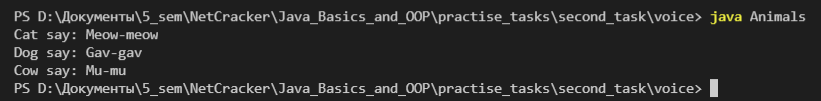
\includegraphics[scale = 0.6]{test_t1.png}
                \label{p2} %% метка рисунка для ссылки на него
            \end{center}
        \end{figure}
    
    \item Чтобы перейти к реализации программы на Github, нажмите на название задачи в самом начале ее описания.
    
\end{enumerate}

\section{\href{https://github.com/julproh/5_sem/tree/main/NetCracker/Java_Basics_and_OOP/practise_tasks/second_task/bones}{Игра в кости}} 

    \begin{enumerate}
        \item \textbf{Задача.} Переработать задачу про игру в кости под использование интерфейсов. 
        Играют N игроков (компьютер в списке последний). Подкидываются 
        одновременно К кубиков. Выигрывает тот, у кого большая сумма очков. 
        Кто выиграл, тот и кидает первым в следующем кону. Игра идет до 7 
        выигрышей. Начинаете игру Вы.

        \item Реализация программы:
        \item Game.java:
        \begin{lstlisting}
            import java.util.Scanner;

            public interface Game {
            
                int getPlayers (Scanner in);
                int getBones (Scanner in);
                int[][] createArray (int n);
                int game(int[][] players, int n, int k);
            
            }
        \end{lstlisting}

        \item Main.java:
        
        \begin{lstlisting}
            import java.util.Random;
            import java.util.Scanner;

            class Bones implements Game{

                @Override
                public int getPlayers (Scanner in) {
                    int n;
                    System.out.println("Print the number of the players with the computer");
                    //Scanner in = new Scanner(System.in);
                    n = in.nextInt();
                    //in.close();
                    return n;
                }

                @Override
                public int getBones (Scanner in) {
                    int k;
                    System.out.println("Print the number of the bones");
                    //Scanner inn = new Scanner(System.in);
                    k = in.nextInt();
                    //inn.close();
                    return k;
                }

                @Override
                public int[][] createArray (int n) {
                    int[][] players = new int[2][n];
                    for  (int i = 0; i < n; i++) {
                        players[0][i] = i+1;
                        players[1][i] = 0;
                    }
                    return players;
                }

                @Override
                public int game(int[][] players, int n, int k) {
                    
                    int[] current = new int [n];
                    int winner = 0;
                    int max = 0;
                    int flag = 0;

                    final Random random = new Random();

                    while (flag == 0) {
                        for (int i = 0; i < n; i++){
                            for (int j = 0; j < k; j++) {
                                
                                current[i] += random.nextInt(5) + 1; 
                            }
                            if ( current[i] > max) {
                                max = current[i];
                                winner = i;
                            }
                        };
                        players[1][winner]++;
                        if (players[1][winner]==7){
                            flag = 1;
                        } 
                        else {
                            int number = players[1][winner];
                            for(int i = winner; i > 0; i--) {
                                players[0][i] = players[0][i-1];
                                players[1][i] = players[1][i-1];
                            }
                            players[0][0] = winner+1;
                            players[1][0] = number;
                            for (int i=0; i < n; i++) {
                                current[i] = 0;
                            }

                        }
                    };
                    return players[0][0];
                }

            }

            public class Main {

                public static void main (String[] args) {

                    Scanner in = new Scanner(System.in);
                    Bones bones = new Bones();
                    int n = bones.getPlayers(in);
                    int k = bones.getBones(in);
                    in.close();

                    int[][] players = bones.createArray(n);

                    int winner = bones.game(players, n, k);

                    System.out.println("The winner is " + winner + " player");

                };
            }
        \end{lstlisting}
    
    \item Результаты тестов:
        
        \begin{figure}[h!]
            \begin{center}
                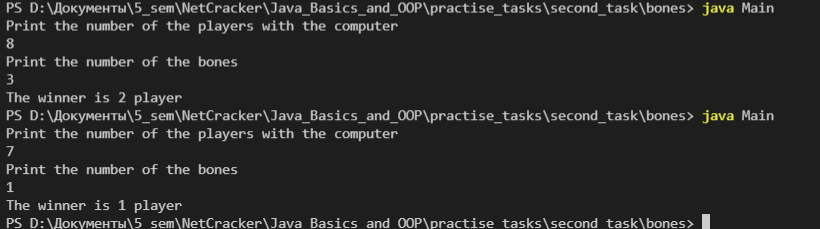
\includegraphics[scale = 0.8]{test_t2.png}
                \label{p2} %% метка рисунка для ссылки на него
            \end{center}
        \end{figure}

    \item Чтобы перейти к реализации программы на Github, нажмите на название задачи в самом начале ее описания.
    
    \end{enumerate}

\section{\href{https://github.com/julproh/5_sem/tree/main/NetCracker/Java_Basics_and_OOP/practise_tasks/second_task/extended}{Extended Class}}

    \begin{enumerate}
   
        \item \textbf{Задача.} Написать программу, реализующую изображенный класс:
        
        \begin{figure}[h!]
            \begin{center}
                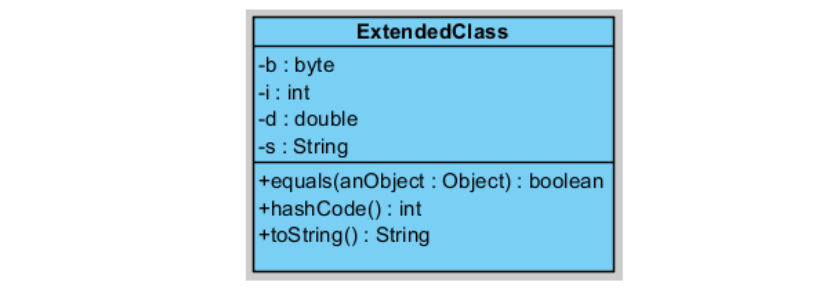
\includegraphics[scale = 0.8]{task.png}
                \label{p2} %% метка рисунка для ссылки на него
            \end{center}
        \end{figure}

        \item Реализация программы:
        \item ExtendedClass.java :
        
        \begin{lstlisting}
            import java.util.Objects;

            public class ExtendedClass {
                byte b;
                int i;
                double d;
                String s;

                @Override
                public boolean equals(Object anObject) {
                    if (anObject == this) {
                        return true;
                    } else if (anObject == null || anObject.getClass() != this.getClass()) {
                        return false;
                    }

                    ExtendedClass extendedClass = (ExtendedClass) anObject;
                    if (this.b == extendedClass.b && this.i  == extendedClass.i && this.d == extendedClass.d && this.s == extendedClass.s) {
                        return true;
                    } 
                    else {
                        return false;
                    }    
                }

                @Override
                public int hashCode() {
                    int result = Objects.hashCode(b);
                    result = 31 * result + Objects.hashCode(i);
                    result = 31 * result + Objects.hashCode(d);
                    result = 31 * result + Objects.hashCode(s);
                    return result;
                }

                @Override
                public String toString() {

                    return "byte: "+ b + "\n" + "int: " +"i "+ "\n" + "double: " + d + "\n" + "String: " + s ;
                }
            }
        \end{lstlisting}

        \item Main.java :
        
        \begin{lstlisting}
            import java.util.Objects;

            public class Main {
            public static void main(String[] args) {

                ExtendedClass extended1 = new ExtendedClass();
                extended1.b = 1;
                extended1.i = 1;
                extended1.d = 0.2;
                extended1.s = "extended";

                ExtendedClass extended2 = new ExtendedClass();
                extended2.b = 1;
                extended2.i = 1;
                extended2.d = 0.2;
                extended2.s = "extended";

                ExtendedClass extended3 = new ExtendedClass();
                extended3.b = 0;
                extended3.i = 1;
                extended3.d = 0.2;
                extended3.s = "extended3";

                String s = "String";

                System.out.println(extended1.equals(extended1));
                System.out.println(extended1.equals(extended2));
                System.out.println(extended1.equals(extended3));
                System.out.println(extended1.equals(s));

                System.out.println("-------------------");

                System.out.println(extended1.hashCode() == extended1.hashCode());
                System.out.println(extended1.hashCode() == extended2.hashCode());
                System.out.println(extended1.hashCode() == extended3.hashCode());
                System.out.println(extended1.hashCode() == s.hashCode());

                System.out.println("-------------------");
                System.out.println(extended3.toString());
                
            }
        }
        \end{lstlisting}

        \item Результаты тестов:
        
        \begin{figure}[h!]
            \begin{center}
                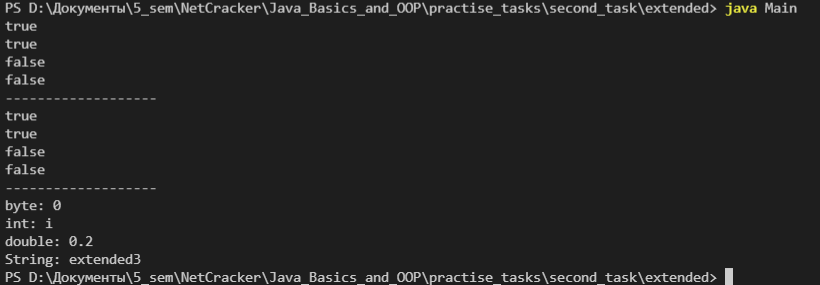
\includegraphics[scale = 0.6]{test_t3.png}
                \label{p2} %% метка рисунка для ссылки на него
            \end{center}
        \end{figure}

        \item Чтобы перейти к реализации программы на Github, нажмите на название задачи в самом начале ее описания.
    
    \end{enumerate}

    \section{\href{https://github.com/julproh/5_sem/tree/main/NetCracker/Java_Basics_and_OOP/practise_tasks/second_task/black}{Black}}

    \begin{enumerate}
        \item \textbf{Задача.} Создать интерфейс Black с методами setColor(String color) и isBlack(). Реализовать интерфейс в классе BlackImpl. Метод setColor(String color) должен устанавливать текущий цвет в color.
         Метод isBlack() должен печатать в консоль "It is black", если текущий цвет == "black", и "it isn't black"  в противном случае.
        \item Реализация программы:
        \item Black.java :
        
        \begin{lstlisting}
            public interface Black{

                void setColor(String color);
                void isBlack();
            }
        \end{lstlisting}

        \item BlackImpl.java :
        
        \begin{lstlisting}
            public class BlackImpl implements Black {
                String color;

                @Override
                public void setColor(String color) {
                    this.color=color;
                }

                @Override
                public void isBlack() {
                    if (this.color == "black"){
                        System.out.println("It is black");
                    }
                    else {
                        System.out.println("It isn't black");
                    }
                }
            }
        \end{lstlisting}

        \item Main.java :
        
        \begin{lstlisting}
            public class Main{
                public static void  main(String[] args) {
                    Black black = new BlackImpl();
                    
                    black.setColor("blue");
                    black.isBlack();

                    black.setColor("black");
                    black.isBlack();
                }
            }
        \end{lstlisting}
        
        \item Результаты тестов:
        
        \begin{figure}[h!]
            \begin{center}
                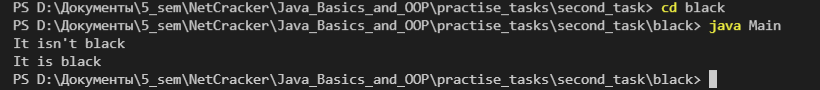
\includegraphics[scale = 0.6]{test_t4.png}
                \label{p2} %% метка рисунка для ссылки на него
            \end{center}
        \end{figure}

        \item Чтобы перейти к реализации программы на Github, нажмите на название задачи в самом начале ее описания.
        
    \end{enumerate}

    \section{Вывод}
    СВ ходе выполнения практического задания были сформированы навыки проектирования и реализации интерфейсов Java, закреплены навыки в области разработки классов java и переопределены методы equals(), hashCode(), toString().

\end{document}